\documentclass{article}

\usepackage{graphicx}
\usepackage{tikz}
\usepackage{tikzsymbols}
\usetikzlibrary{calc,patterns,shapes.geometric}
\pagestyle{empty}
\usepackage[margin=0pt]{geometry}
\geometry{papersize={14in,12in}}

\def\centerarc[#1](#2)(#3:#4:#5){\draw[#1] ($(#2)+({#5*cos(#3)},{#5*sin(#3)})$) arc (#3:#4:#5);}

\begin{document}
	\begin{figure}
		\centering
		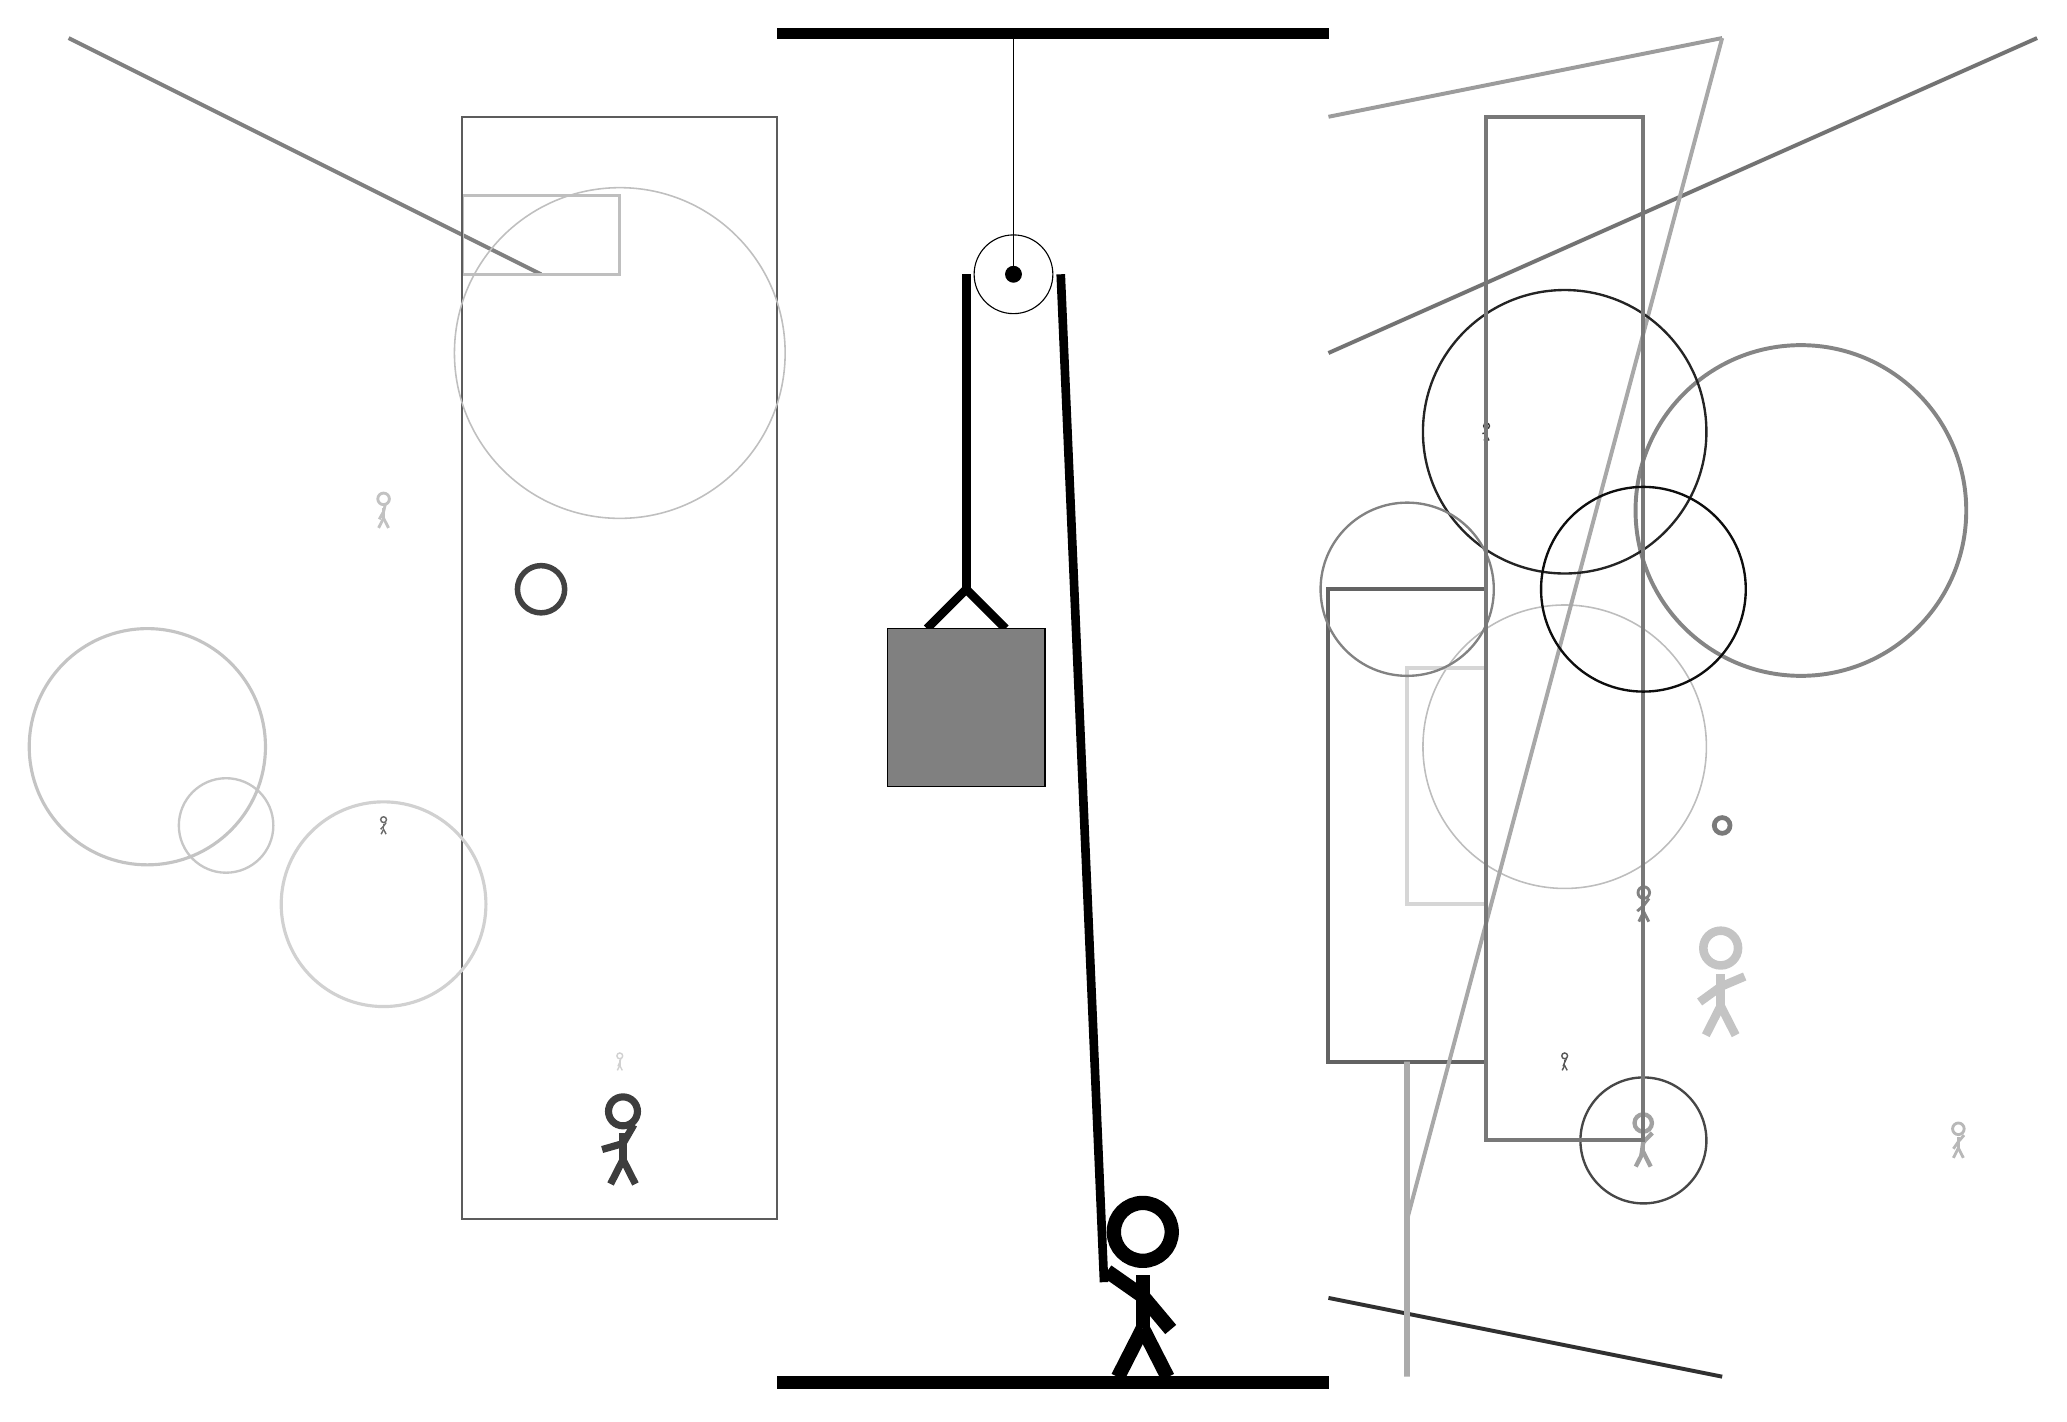
\begin{tikzpicture}
			%%%%% START %%%%%
			
			\draw[fill=black] (-2, 14) rectangle (5, 14.125);
			
			\draw (1, 11) circle (0.5);
			\draw[fill=black] (1, 11) circle (0.1);
			\draw (1, 14) -- (1, 11);
			
			\draw[line width=0.5mm, color=black!55](5, 10) -- (14, 14);
			
			\draw [line width=0.6mm, color=black!52](10, 4) circle (0.1);
			\draw [line width=0.3mm, color=black!22](-9, 4) circle (0.6);
			\node[line width=0.4mm, color=black!79] at (7, 9) {\Strichmaxerl[1][17][81]};
			
			\draw[line width=0.5mm, color=black!50](-5, 11) -- (-11, 14);
			
			\node[line width=0.7mm, color=black!49] at (9, 3) {\Strichmaxerl[2][41][53]};
			\node[line width=0.4mm, color=black!58] at (-7, 4) {\Strichmaxerl[1][48][54]};
			\draw[line width=0.5mm, color=black!61] (7, 1) rectangle (5, 7);
			\node[line width=0.3mm, color=black!23] at (10, 2) {\Strichmaxerl[6][36][23]};
			\node[line width=0.2mm, color=black!28] at (13, 0) {\Strichmaxerl[2][55][49]};
			
			\node[line width=0.2mm, color=black!65] at (8, 1) {\Strichmaxerl[1][68][64]};
			\draw [line width=0.4mm, color=black!23](-10, 5) circle (1.5);
			\draw[line width=0.4mm, color=black!25] (-4, 11) rectangle (-6, 12);
			
			\draw [line width=0.5mm, color=black!48](11, 8) circle (2.1);
			\draw [line width=0.7mm, color=black!74](-5, 7) circle (0.3);
			\draw[line width=0.3mm, color=black!64] (-2, -1) rectangle (-6, 13);
			\draw [line width=0.2mm, color=black!26](8, 5) circle (1.8);
			
			\node[line width=0.3mm, color=black!37] at (9, 0) {\Strichmaxerl[3][82][46]};
			\draw[line width=0.5mm, color=black!16] (7, 6) rectangle (6, 3);
			
			\draw[line width=0.5mm, color=black!81](10, -3) -- (5, -2);
			\draw[line width=0.5mm, color=black!39](5, 13) -- (10, 14);
			\draw[line width=0.5mm, color=black!34](6, -1) -- (10, 14);
			
			\node[line width=0.6mm, color=black!76] at (-4, 0) {\Strichmaxerl[5][16][60]};
			\draw [line width=0.3mm, color=black!86](8, 9) circle (1.8);
			\draw [line width=0.4mm, color=black!18](-7, 3) circle (1.3);
			
			\draw[line width=0.7mm, color=black!33] (6, -3) rectangle (6, 1);
			\draw [line width=0.3mm, color=black!72](9, 0) circle (0.8);
			\draw [line width=0.3mm, color=black!49](6, 7) circle (1.1);
			
			\draw [line width=0.2mm, color=black!25](-4, 10) circle (2.1);
			\draw[line width=0.5mm, color=black!53] (7, 0) rectangle (9, 13);
			\draw [line width=0.3mm, color=black!95](9, 7) circle (1.3);
			
			\node[line width=0.7mm, color=black!18] at (-4, 1) {\Strichmaxerl[1][65][74]};
			\node[line width=0.3mm, color=black!24] at (-7, 8) {\Strichmaxerl[2][60][77]};
			
			
			\draw[line width=1.1mm] (-0.1, 6.5) -- (0.4, 7.0) -- (0.9, 6.5);
			\draw[fill=black!50] (-0.6, 6.5) rectangle (1.4, 4.5);
			
			\draw[line width=1.1mm] (0.4, 11) -- (0.4, 7.0);
			\centerarc[line width=1.1mm](1, 11)(0:180:0.6);
			\draw[line width=1.1mm](1.6, 11) -- (2.15, -1.8);
			
			\node at (2.6, -1.9) {\Strichmaxerl[10][-35][-50]};
			
			\draw[fill=black] (-2, -3) rectangle (5, -3.15);
			
			%%%%% END %%%%%
		\end{tikzpicture}
	\end{figure}	
\end{document}